\chapter{Introduction to \texttt{python}}\label{introduction-to-python---lesson-1}

$\tt{Python}$ is one of the most widely used programming languages in the world, and it has been around for more than 28 years now~\cite{survey2019}.

First and foremost reason why $\tt{python}$ is much popular because it is highly productive as compared to other programming languages like $\tt{C++}$ and $\tt{java}$. It is a much more concise and expressive language and requires less time, effort, and lines of code to perform the same operations.

This makes $\tt{python}$ very easy-to-learn programming language even for beginners and newbies. It is also very famous for its simple programming syntax, code readability and English-like commands that make coding in \texttt{python} lot easier and efficient.
With $\tt{python}$, the code looks very close to how humans think. For this purpose, it must abstract the details of the computer from you. Hence, it is slower than other “lower-level language” like $\tt{C}$.

There were times when computer run time was to be the main issue and the most expensive resource. But now, things have changed. Computer, servers and other hardware have become much much cheaper than ever and speed has become a less important factor. Today, development time matters more in most cases rather than execution speed. Reducing the time needed for each project saves companies tons of money.

As far as the execution speed or performance of the program is concerned, we can easily manage it by horizontal scaling, meaning that more servers can be used to reach that level of speed or performance.

In short, $\tt{python}$ is widely used even when it is somehow slower than other languages because:
\begin{itemize}
  \item is more productive;
  \item companies can optimize their most expensive resource: employees;
  \item rich set of libraries and frameworks;
  \item large community.
\end{itemize}


\begin{center}
  \begin{figure}
    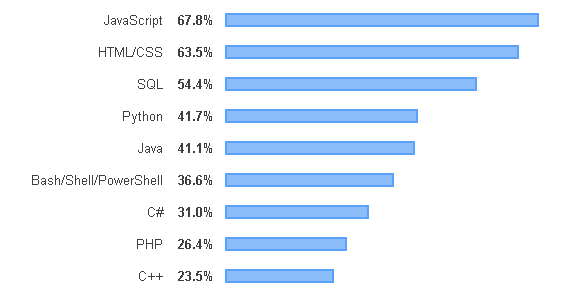
\includegraphics[width=0.7\linewidth]{figures/most_used}
    \caption{List of most used languages by developers according to Stack Overflow survey in 2019.}
  \end{figure}
  \begin{figure}
    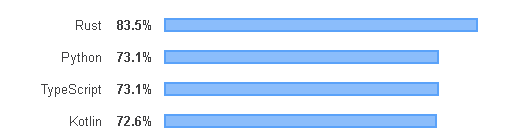
\includegraphics[width=0.7\linewidth]{figures/most_loved}
    \caption{List of most loved languages by developers according to Stack Overflow survey in 2019.}
  \end{figure}
  \begin{figure}
    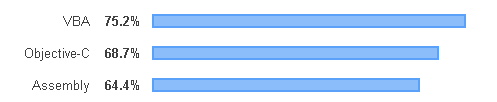
\includegraphics[width=0.7\textwidth]{figures/most_dreaded}
    \caption{List of most \emph{dreaded} languages by developers according to Stack Overflow survey in 2019.}
  \end{figure}
\end{center}

\section{What is $\tt{python}$ ?}\label{what-is-python}

$\tt{python}$ is a so called \emph{interpreted language}: it takes some code (a sequence of instructions), reads and executes it. This is different from other programming languages like \texttt{C} or \texttt{C++} which \emph{compile} code into a language that the computer can understand directly (\emph{machine language}).

\begin{figure}[h]
\centering
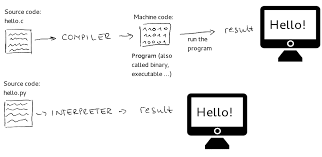
\includegraphics[width=0.7\linewidth]{figures/index.png}
\caption{Interpreted vs compiled language}
\end{figure}

As a result, \(\tt{python}\) is essentially an \emph{interactive} programming language, you can program and see the results almost at the same time. This is very nice for a faster development since compilation time can be quite long (just to give an idea the compilation of our \texttt{C++} financial code takes more than one hour).
However there are drawbacks in terms of performance, the \emph{translation} to machine language has to be done in real-time resulting in slower execution times.

\begin{figure}[h]
\centering
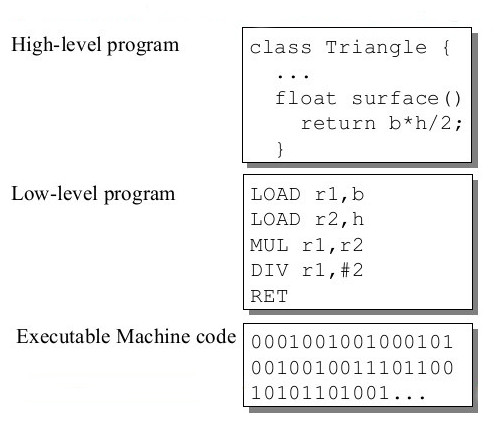
\includegraphics[width=0.5\linewidth]{figures/machine_language.jpeg}
\caption{Human readable vs machine code}
\end{figure}

In the next chapters we'll take a quick tour of $\tt{python}$ and see the main features and characteristics of this programming language, later on we will see how it can be useful to solve real-world financial problems.

First of all since $\tt{python}$, as basically all programs, comes in different version and flavours we need to specify the particular one we are going to use~\cite{python_versions}.
The latest version (at the time I'm writing this pages) is \(\tt{3.8.5}\), but it is continuously evolving, however it is not difficult to see older versions floating around (e.g. \(\tt{2.7}\)).
This is because there are some big differences between \(\tt{python 2.X}\) and \(\tt{python 3.X}\) which prevent a sizable portion of \(\tt{python 2}\) users to stick with it (consider that moving to \(\tt{python 3}\) would require a large amount of work to adapt big projects).
In conclusion we will concentrate on \textbf{\(\tt{python~3.7}\)}.

\section{$\tt{python}$ basics}\label{python-basics}

Every language has \emph{keywords}, these are reserved words that have a special meaning and tell the computer what to do. The first one we encounter is \(\tt{print}\): it prints to screen whatever is specified between the parenthesis.

\begin{tcolorbox}[breakable, size=fbox, boxrule=1pt, pad at break*=1mm, colback=cellbackground, colframe=cellborder]
\begin{Verbatim}[commandchars=\\\{\}]
\PY{n+nb}{print} \PY{p}{(}\PY{l+s+s2}{\PYZdq{}}\PY{l+s+s2}{Hello world !}\PY{l+s+s2}{\PYZdq{}}\PY{p}{)} 

Hello world !
\end{Verbatim}
\end{tcolorbox}

\begin{tcolorbox}[breakable, size=fbox, boxrule=1pt, pad at break*=1mm, colback=cellbackground, colframe=cellborder]
\begin{Verbatim}[commandchars=\\\{\}]
\PY{n+nb}{print} \PY{p}{(}\PY{l+s+s2}{\PYZdq{}}\PY{l+s+s2}{Welcome}\PY{l+s+s2}{\PYZdq{}}\PY{p}{)}
\PY{n+nb}{print} \PY{p}{(}\PY{l+s+s2}{\PYZdq{}}\PY{l+s+s2}{to}\PY{l+s+s2}{\PYZdq{}}\PY{p}{)}
\PY{n+nb}{print} \PY{p}{(}\PY{l+s+s2}{\PYZdq{}}\PY{l+s+s2}{everybody}\PY{l+s+s2}{\PYZdq{}}\PY{p}{)}

Welcome
to
everybody
\end{Verbatim}
\end{tcolorbox}

Good programming practice recommends to document the code you write (you will soon see that it is surprisingly easy to forget what you wanted to do in your code). In \(\tt{python}\) you can add comments to code starting a line with a hash character (\#).

\begin{tcolorbox}[breakable, size=fbox, boxrule=1pt, pad at break*=1mm, colback=cellbackground, colframe=cellborder]
\begin{Verbatim}[commandchars=\\\{\}]
\PY{n+nb}{print} \PY{p}{(}\PY{l+s+s2}{\PYZdq{}}\PY{l+s+s2}{Ciao}\PY{l+s+s2}{\PYZdq{}}\PY{p}{)} \PY{c+c1}{\PYZsh{} this is a comment}

Ciao
\end{Verbatim}
\end{tcolorbox}

\subsection{Variables}\label{variables}

A variable is a computer memory location paired with a symbolic name, which contains some quantity of information referred to as a *value* (e.g.~a number, a string\ldots{}). Variables and hence data they contain, can be used, referenced and manipulated throughout a program.
A value is assigned to a variable with the equal operator (=) and printing a variable shows its content. 

\begin{figure}[h]
\centering
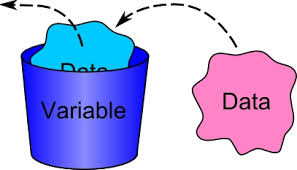
\includegraphics[width=0.35\linewidth]{figures/var1.jpeg}\\
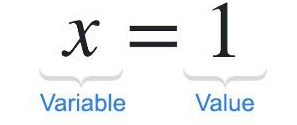
\includegraphics[width=0.35\linewidth]{figures/var2.jpeg}
\caption{Graphical representation of a variable.}
\end{figure}

\begin{tcolorbox}[breakable, size=fbox, boxrule=1pt, pad at break*=1mm, colback=cellbackground, colframe=cellborder]
\begin{Verbatim}[commandchars=\\\{\}]
\PY{n}{x} \PY{o}{=} \PY{l+m+mi}{9}
\PY{n+nb}{print} \PY{p}{(}\PY{n}{x}\PY{p}{)}

9
\end{Verbatim}
\end{tcolorbox}

\begin{tcolorbox}[breakable, size=fbox, boxrule=1pt, pad at break*=1mm, colback=cellbackground, colframe=cellborder]
\begin{Verbatim}[commandchars=\\\{\}]
\PY{n}{myphone} \PY{o}{=} \PY{l+s+s2}{\PYZdq{}}\PY{l+s+s2}{Huawei P10Lite}\PY{l+s+s2}{\PYZdq{}}
\PY{n+nb}{print} \PY{p}{(}\PY{n}{myphone}\PY{p}{)}

Huawei P10Lite
\end{Verbatim}
\end{tcolorbox}

Another very useful keyword is \(\tt{type}\): it tells which kind of object is stored in a variable.

\begin{tcolorbox}[breakable, size=fbox, boxrule=1pt, pad at break*=1mm, colback=cellbackground, colframe=cellborder]
\begin{Verbatim}[commandchars=\\\{\}]
\PY{n+nb}{print} \PY{p}{(}\PY{n+nb}{type}\PY{p}{(}\PY{n}{x}\PY{p}{)}\PY{p}{)}
\PY{n+nb}{print} \PY{p}{(}\PY{n+nb}{type}\PY{p}{(}\PY{n}{myphone}\PY{p}{)}\PY{p}{)}

<class 'int'>
<class 'str'>
\end{Verbatim}
\end{tcolorbox}

After their definitions \(\tt{x}\) and \(\tt{myphone}\) can be used as aliases for a number and a string and their content manipulated, for example:

\begin{tcolorbox}[breakable, size=fbox, boxrule=1pt, pad at break*=1mm, colback=cellbackground, colframe=cellborder]
\begin{Verbatim}[commandchars=\\\{\}]
\PY{n+nb}{print} \PY{p}{(}\PY{n}{x}\PY{o}{+}\PY{l+m+mi}{5}\PY{p}{)}

14
\end{Verbatim}
\end{tcolorbox}

There are rules that limit the variable naming possibilities, in particular they must:
\begin{itemize}
\item begin with a letter (\texttt{myphone}) or underscore (\texttt{\_myphone});
\item other characters can be letters, numbers or more \_;
\item variable names are case-sensitive so \texttt{myphone} and \texttt{myPhone} are two distinct variables;
\end{itemize}

\textbf{Keywords, as said, are reserved words and as such cannot be used as variable names (e.g.~\texttt{print, type, for...})}.

To use \textbf{good} variable names (and make your programs clearer and easier to read) always choose meaningful names instead of short names (i.e. \texttt{numberOfCakes} is much better than simply \texttt{n}), try to be consistent with your conventions (e.g.~choose once and for all between \texttt{number\_of\_cakes} or \texttt{numberofcakes} or \texttt{numberOfCakes}, usually begin a variable name with underscore (\_) only for a special case (will see later when this is usually done).

\subsection{Boolean expressions}\label{boolean-expressions}

Boolean expressions evaluate to \(\tt{true}\) or \(\tt{false}\) only. This type
of expressions usually involve logical or comparison operators like \(\tt{or}\), \(\tt{and}\), \textgreater{} (greater-than), \textless{} (less-than),\ldots{}
The equal-to Boolean operator symbol is a double = (==), to not be confused with the assignment operator single = (=), with the first we compare two variables, with the second we associate a value to a variable.

Let's see some example. The following expression answers the question is 1 equal to 2:

\begin{tcolorbox}[breakable, size=fbox, boxrule=1pt, pad at break*=1mm, colback=cellbackground, colframe=cellborder]
\begin{Verbatim}[commandchars=\\\{\}]
\PY{l+m+mi}{1} \PY{o}{==} \PY{l+m+mi}{2} 

False
\end{Verbatim}
\end{tcolorbox}

Here another example using the not equal operator (!=):

\begin{tcolorbox}[breakable, size=fbox, boxrule=1pt, pad at break*=1mm, colback=cellbackground, colframe=cellborder]
\begin{Verbatim}[commandchars=\\\{\}]
\PY{l+m+mi}{1} \PY{o}{!=} \PY{l+m+mi}{2}
  
True
\end{Verbatim}
\end{tcolorbox}

\begin{tcolorbox}[breakable, size=fbox, boxrule=1pt, pad at break*=1mm, colback=cellbackground, colframe=cellborder]
\begin{Verbatim}[commandchars=\\\{\}]
\PY{l+m+mi}{2} \PY{o}{\PYZlt{}} \PY{l+m+mi}{2}

False
\end{Verbatim}
\end{tcolorbox}

\begin{tcolorbox}[breakable, size=fbox, boxrule=1pt, pad at break*=1mm, colback=cellbackground, colframe=cellborder]
\begin{Verbatim}[commandchars=\\\{\}]
\PY{l+m+mi}{2} \PY{o}{\PYZlt{}}\PY{o}{=} \PY{l+m+mi}{2}  \PY{c+c1}{\PYZsh{} in this case we allow the numbers to be equal too}

True
\end{Verbatim}
\end{tcolorbox}

\begin{tcolorbox}[breakable, size=fbox, boxrule=1pt, pad at break*=1mm, colback=cellbackground, colframe=cellborder]
\begin{Verbatim}[commandchars=\\\{\}]
\PY{n+nb}{print} \PY{p}{(}\PY{n}{x}\PY{p}{)}
\PY{l+m+mi}{15} \PY{o}{\PYZlt{}}\PY{o}{=} \PY{n}{x} \PY{o+ow}{and} \PY{n}{x} \PY{o}{\PYZlt{}}\PY{o}{=} \PY{l+m+mi}{20} \PY{c+c1}{\PYZsh{} this expression could also be written as 15 \PYZlt{}= x \PYZlt{}= 20}

11
False
\end{Verbatim}
\end{tcolorbox}

\begin{tcolorbox}[breakable, size=fbox, boxrule=1pt, pad at break*=1mm, colback=cellbackground, colframe=cellborder]            
\begin{Verbatim}[commandchars=\\\{\}]
\PY{l+m+mi}{15} \PY{o}{\PYZlt{}}\PY{o}{=} \PY{n}{x} \PY{o+ow}{or} \PY{n}{x} \PY{o}{\PYZlt{}}\PY{o}{=} \PY{l+m+mi}{20}

True
\end{Verbatim}
\end{tcolorbox}

\begin{tcolorbox}[breakable, size=fbox, boxrule=1pt, pad at break*=1mm, colback=cellbackground, colframe=cellborder]            
\begin{Verbatim}[commandchars=\\\{\}]
\PY{o+ow}{not} \PY{p}{(}\PY{n}{x} \PY{o}{\PYZgt{}} \PY{l+m+mi}{20}\PY{p}{)} \PY{c+c1}{\PYZsh{} the not keyword negates the following expression}

True
\end{Verbatim}
\end{tcolorbox}

\subsection{String expressions}\label{string-expressions}

A ``string'' is a sequence of characters (letters, digits, spaces, punctuation,\ldots). There are many operations that can be performed on strings, like for example concatenate (with + operator), truncate, replace characters,\ldots

\begin{tcolorbox}[breakable, size=fbox, boxrule=1pt, pad at break*=1mm, colback=cellbackground, colframe=cellborder]            
\begin{Verbatim}[commandchars=\\\{\}]
\PY{n}{mystring} \PY{o}{=} \PY{l+s+s2}{\PYZdq{}}\PY{l+s+s2}{some text with punctuation, spaces and digits 10}\PY{l+s+s2}{\PYZdq{}}
\PY{n}{mystring}\PY{o}{.}\PY{n}{replace}\PY{p}{(}\PY{l+s+s2}{\PYZdq{}}\PY{l+s+s2}{s}\PY{l+s+s2}{\PYZdq{}}\PY{p}{,} \PY{l+s+s2}{\PYZdq{}}\PY{l+s+s2}{z}\PY{l+s+s2}{\PYZdq{}}\PY{p}{)}

'zome text with punctuation, zpacez and digitz 10'
\end{Verbatim}
\end{tcolorbox}

\begin{tcolorbox}[breakable, size=fbox, boxrule=1pt, pad at break*=1mm, colback=cellbackground, colframe=cellborder]            
\begin{Verbatim}[commandchars=\\\{\}]
\PY{l+s+s2}{\PYZdq{}}\PY{l+s+s2}{abc}\PY{l+s+s2}{\PYZdq{}} \PY{o}{+} \PY{l+s+s2}{\PYZdq{}}\PY{l+s+s2}{def}\PY{l+s+s2}{\PYZdq{}} \PY{c+c1}{\PYZsh{} it is possible to concatenate strings with + }

'abcdef'
\end{Verbatim}
\end{tcolorbox}

\begin{tcolorbox}[breakable, size=fbox, boxrule=1pt, pad at break*=1mm, colback=cellbackground, colframe=cellborder]            
\begin{Verbatim}[commandchars=\\\{\}]
\PY{l+s+s2}{\PYZdq{}}\PY{l+s+s2}{The number }\PY{l+s+s2}{\PYZdq{}} \PY{o}{+} \PY{l+m+mi}{4} \PY{o}{+} \PY{l+s+s2}{\PYZdq{}}\PY{l+s+s2}{ is my favourite number}\PY{l+s+s2}{\PYZdq{}}
\PY{c+c1}{\PYZsh{} this causes an error since we are trying to concatenate a string }
\PY{c+c1}{\PYZsh{} with a number so two different kind of objects}

---------------------------------------------------------------------------

TypeError                                 Traceback (most recent call last)

<ipython-input-33-b9f65c5a45f7> in <module>()
----> 1 "The number " + 4 + " is my favourite number"
      2 \# this causes an error since we are trying to concatenate a string
      3 \# with a number so two different kind of objects

TypeError: can only concatenate str (not "int") to str
\end{Verbatim}
\end{tcolorbox}

To avoid this error is possible to \textbf{cast} an object to a different type which means to convert an object to a different type. In this case we can \emph{force} the number four to be represented as a string with the \(\tt{str()}\) function:

\begin{tcolorbox}[breakable, size=fbox, boxrule=1pt, pad at break*=1mm, colback=cellbackground, colframe=cellborder]            
\begin{Verbatim}[commandchars=\\\{\}]
\PY{l+s+s2}{\PYZdq{}}\PY{l+s+s2}{The number }\PY{l+s+s2}{\PYZdq{}} \PY{o}{+} \PY{n+nb}{str}\PY{p}{(}\PY{l+m+mi}{4}\PY{p}{)} \PY{o}{+} \PY{l+s+s2}{\PYZdq{}}\PY{l+s+s2}{ is my favourite number}\PY{l+s+s2}{\PYZdq{}}

'The number 4 is my favourite number'
\end{Verbatim}
\end{tcolorbox}

\begin{tcolorbox}[breakable, size=fbox, boxrule=1pt, pad at break*=1mm, colback=cellbackground, colframe=cellborder]            
\begin{Verbatim}[commandchars=\\\{\}]
\PY{n+nb}{print} \PY{p}{(}\PY{n+nb}{type}\PY{p}{(}\PY{l+m+mf}{3.4}\PY{p}{)}\PY{p}{)}
\PY{n+nb}{print} \PY{p}{(}\PY{n+nb}{type}\PY{p}{(}\PY{n+nb}{str}\PY{p}{(}\PY{l+m+mf}{3.4}\PY{p}{)}\PY{p}{)}\PY{p}{)}

<class 'float'>
<class 'str'>
\end{Verbatim}
\end{tcolorbox}

In this simple case everything worked fine but type casting is not always possible: for example a number can be converted to a string (e.g.~from the integer 4 to the actual symbol ``4'') but the opposite is not possible (e.g.~cannot convert the string ``matteo'' to a meaningful number). In this second case we can try to use the function \(\tt{int()}\) to convert a string to an integer.

\begin{tcolorbox}[breakable, size=fbox, boxrule=1pt, pad at break*=1mm, colback=cellbackground, colframe=cellborder]            
\begin{Verbatim}[commandchars=\\\{\}]
\PY{n+nb}{int}\PY{p}{(}\PY{l+s+s2}{\PYZdq{}}\PY{l+s+s2}{matteo}\PY{l+s+s2}{\PYZdq{}}\PY{p}{)}

---------------------------------------------------------------------------

ValueError                                Traceback (most recent call last)

<ipython-input-17-979283bb65e4> in <module>
----> 1 int("matteo")  

ValueError: invalid literal for int() with base 10: 'matteo'
\end{Verbatim}
\end{tcolorbox}

\begin{tcolorbox}[breakable, size=fbox, boxrule=1pt, pad at break*=1mm, colback=cellbackground, colframe=cellborder]            
\begin{Verbatim}[commandchars=\\\{\}]
\PY{n+nb}{int}\PY{p}{(}\PY{l+s+s2}{\PYZdq{}}\PY{l+s+s2}{4}\PY{l+s+s2}{\PYZdq{}}\PY{p}{)}

4
\end{Verbatim}
\end{tcolorbox}

\subsubsection{Pretty string formatting}
In order to get prettier strings than those obtained just concatenating with the + operator, \texttt{python} allows to format text using the following syntax \texttt{"text \{\} other text \{\}".format(var1, var2)}.
With this notation, each \texttt{\{\}} is mapped to the variables listed in the \texttt{format} statement, the optional characters inside the curly brackets can determine the resulting format, for example in the following code \texttt{\{:.1f\}} means that this variable is a float number and that has to be printed with only one digit only after the decimal separator. 

\begin{tcolorbox}[breakable, size=fbox, boxrule=1pt, pad at break*=1mm, colback=cellbackground, colframe=cellborder]            
\begin{Verbatim}[commandchars=\\\{\}]
\PY{l+s+s2}{\PYZdq{}}\PY{l+s+s2}{The speed of light is about }\PY{l+s+si}{\PYZob{}:.1f\PYZcb{}}\PY{l+s+s2}{ }\PY{l+s+si}{\PYZob{}\PYZcb{}}\PY{l+s+s2}{\PYZdq{}}\PY{o}{.}\PY{n}{format}\PY{p}{(}\PY{l+m+mf}{299792.458}\PY{p}{,} \PY{l+s+s2}{\PYZdq{}}\PY{l+s+s2}{km/s}\PY{l+s+s2}{\PYZdq{}}\PY{p}{)}

'The speed of light is about 299792.5 km/s'
\end{Verbatim}
\end{tcolorbox}

In addition $\tt{format}$ allows for 0-padding of numbers, left or right alignment of text columns and so on.

\subsection{Mathematical expressions}\label{mathematical-expressions}

Below few examples of the basic mathematical expressions available in $\tt{python}$.

\begin{tcolorbox}[breakable, size=fbox, boxrule=1pt, pad at break*=1mm, colback=cellbackground, colframe=cellborder]            
\begin{Verbatim}[commandchars=\\\{\}]
\PY{l+m+mi}{1} \PY{o}{+} \PY{l+m+mi}{2}

3
\end{Verbatim}
\end{tcolorbox}

\begin{tcolorbox}[breakable, size=fbox, boxrule=1pt, pad at break*=1mm, colback=cellbackground, colframe=cellborder]            
\begin{Verbatim}[commandchars=\\\{\}]
\PY{l+m+mi}{40} \PY{o}{\PYZhy{}} \PY{l+m+mi}{5}

35
\end{Verbatim}
\end{tcolorbox}

\begin{tcolorbox}[breakable, size=fbox, boxrule=1pt, pad at break*=1mm, colback=cellbackground, colframe=cellborder]            
\begin{Verbatim}[commandchars=\\\{\}]
\PY{n}{x} \PY{o}{*} \PY{l+m+mi}{20} \PY{c+c1}{\PYZsh{} remember that we set x equal to 9}

180
\end{Verbatim}
\end{tcolorbox}

\begin{tcolorbox}[breakable, size=fbox, boxrule=1pt, pad at break*=1mm, colback=cellbackground, colframe=cellborder]            
\begin{Verbatim}[commandchars=\\\{\}]
\PY{n}{x} \PY{o}{/} \PY{l+m+mi}{4}

2.25
\end{Verbatim}
\end{tcolorbox}

\begin{tcolorbox}[breakable, size=fbox, boxrule=1pt, pad at break*=1mm, colback=cellbackground, colframe=cellborder]            
\begin{Verbatim}[commandchars=\\\{\}]
\PY{n+nb}{print} \PY{p}{(}\PY{n+nb}{type}\PY{p}{(}\PY{l+m+mf}{2.25}\PY{p}{)}\PY{p}{)}

<class 'float'>
\end{Verbatim}
\end{tcolorbox}

\begin{tcolorbox}[breakable, size=fbox, boxrule=1pt, pad at break*=1mm, colback=cellbackground, colframe=cellborder]            
\begin{Verbatim}[commandchars=\\\{\}]
\PY{n}{x} \PY{o}{/}\PY{o}{/} \PY{l+m+mi}{4} \PY{c+c1}{\PYZsh{} integer division \PYZhy{} result will be truncated to the }
       \PY{c+c1}{\PYZsh{} corresponding integer (no rounding)}
       \PY{c+c1}{\PYZsh{} 11 / 3 = 3.666666 \PYZhy{}\PYZgt{} 11 // 3 = 3}

2
\end{Verbatim}
\end{tcolorbox}

\begin{tcolorbox}[breakable, size=fbox, boxrule=1pt, pad at break*=1mm, colback=cellbackground, colframe=cellborder]            
\begin{Verbatim}[commandchars=\\\{\}]
\PY{n}{y} \PY{o}{=} \PY{l+m+mi}{3}
\PY{n}{x} \PY{o}{*}\PY{o}{*} \PY{n}{y} \PY{c+c1}{\PYZsh{} x to the power of y}

729
\end{Verbatim}
\end{tcolorbox}

\begin{tcolorbox}[breakable, size=fbox, boxrule=1pt, pad at break*=1mm, colback=cellbackground, colframe=cellborder]            
\begin{Verbatim}[commandchars=\\\{\}]
\PY{l+m+mi}{3} \PY{o}{*} \PY{p}{(}\PY{n}{x} \PY{o}{+} \PY{n}{y}\PY{p}{)}

36
\end{Verbatim}
\end{tcolorbox}

As an example of variable manipulation let's try to increment \(\tt{x}\) by 1 and save the result again in \(\tt{x}\).

\begin{tcolorbox}[breakable, size=fbox, boxrule=1pt, pad at break*=1mm, colback=cellbackground, colframe=cellborder]            
\begin{Verbatim}[commandchars=\\\{\}]
\PY{n+nb}{print} \PY{p}{(}\PY{n}{x}\PY{p}{)}
\PY{n}{x} \PY{o}{=} \PY{n}{x} \PY{o}{+} \PY{l+m+mi}{1}
\PY{n+nb}{print} \PY{p}{(}\PY{n}{x}\PY{p}{)}

15
16
\end{Verbatim}
\end{tcolorbox}

Sometimes the increment of a variable plus the assignment to the same variable is written with a more compact syntax \texttt{x += 1} (this is also true for other operators e.g. \texttt{x *= 2}).

More complex mathematical functions are not directly available, let's see for example the logarithm:

\begin{tcolorbox}[breakable, size=fbox, boxrule=1pt, pad at break*=1mm, colback=cellbackground, colframe=cellborder]            
\begin{Verbatim}[commandchars=\\\{\}]
\PY{n}{log}\PY{p}{(}\PY{l+m+mi}{3}\PY{p}{)}

---------------------------------------------------------------------------

NameError                                 Traceback (most recent call last)

<ipython-input-17-ffde4d60496a> in <module>()
    ----> 1 log(3) \# causes an error because the logarithm function
          2        \# is not available by default


NameError: name 'log' is not defined
\end{Verbatim}
\end{tcolorbox}

\section{Modules}\label{modules}

One very important feature of each language is the ability to reuse code among different programs, e.g.~imagine how awful would be if you had to re-implement every time you need it a function to compute the logarithm.
Usually there are mechanisms that allow to collect useful routines in \emph{packages} (or \emph{libraries}, or \emph{modules}) so that later they can be called and used by any program may need them.

These collections of utilities in \(\tt{python}\) are called \emph{modules} and each installation of this language brings with it a standard set of them. If you need more functionality, you can download more modules from the web (there are zillions out there~\cite{modules}) or if you are not satisfied with what you found you can write your own (which is one the goal of this course in the end).

Some examples of useful modules we will use are:

\begin{itemize}
\tightlist
\item
  Numpy - which provides matrix algebra functionality and much more;
\item
  Scipy - which provides a whole series of scientific computing
  functions;
\item
  Pandas - which provides tools for manipulating time series or data-set
  in general;
\item
  Matplotlib - for plotting graphs;
\item
  Jupyter - for notebooks like the one used in classroom.
\end{itemize}

\begin{figure}
\centering
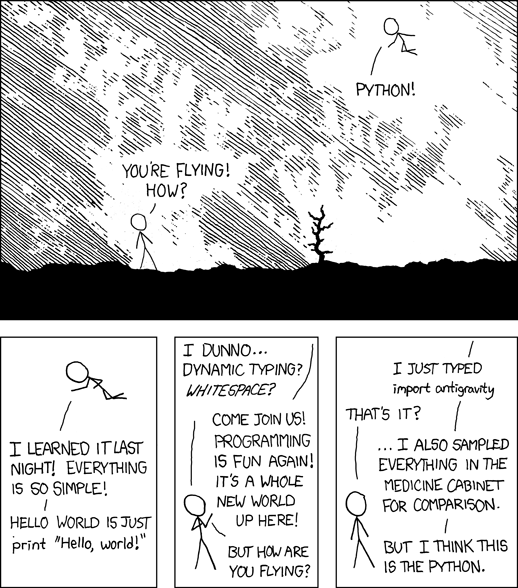
\includegraphics[width=0.5\linewidth]{figures/python.png}
\caption{$\tt{Python}$ has many modules for download on the web\ldots{}}
\end{figure}

Later we will take a closer look at three modules which are quite useful in financial analysis.

In order to load a module in a \(\tt{python}\) program you can use the \(\tt{import}\) keyword. To inspect a module (to understand which are its functionalities) it can be used the \(\tt{help}\) and \(\tt{dir}\) keywords: the first write a help message which usually describes the functionalities of a module, the latter list all the available functions of a module.
\textbf{In order to access a function of a module you have to use the . (dot) operator: \texttt{module-name.function-name}.}

Let's see an example dealing with the \texttt{math} module which implements the most common mathematical functions.

\begin{tcolorbox}[breakable, size=fbox, boxrule=1pt, pad at break*=1mm, colback=cellbackground, colframe=cellborder]            
\begin{Verbatim}[commandchars=\\\{\}]
\PY{k+kn}{import} \PY{n+nn}{math}
\PY{n+nb}{dir}\PY{p}{(}\PY{n}{math}\PY{p}{)}

 ['\_\_doc\_\_',
  '\_\_loader\_\_',
  '\_\_name\_\_',
  '\_\_package\_\_',
  '\_\_spec\_\_',
  'acos',
  'acosh',
  'asin',
  'asinh',
  'atan',
  'atan2',
  'atanh',
  'ceil',
  'copysign',
  'cos',
  'cosh',
...
\end{Verbatim}
\end{tcolorbox}

\begin{tcolorbox}[breakable, size=fbox, boxrule=1pt, pad at break*=1mm, colback=cellbackground, colframe=cellborder]            
\begin{Verbatim}[commandchars=\\\{\}]
\PY{n+nb}{help}\PY{p}{(}\PY{n}{math}\PY{p}{)}

Help on module math:

NAME
    math

MODULE REFERENCE
    https://docs.python.org/3.6/library/math

    The following documentation is automatically generated from the Python
    source files.  It may be incomplete, incorrect or include features that
    are considered implementation detail and may vary between Python
    implementations.  When in doubt, consult the module reference at the
    location listed above.

DESCRIPTION
    This module is always available.  It provides access to the
    mathematical functions defined by the C standard.

FUNCTIONS
    acos({\ldots})
        acos(x)

        Return the arc cosine (measured in radians) of x.
...
\end{Verbatim}
\end{tcolorbox}

\begin{tcolorbox}[breakable, size=fbox, boxrule=1pt, pad at break*=1mm, colback=cellbackground, colframe=cellborder]            
\begin{Verbatim}[commandchars=\\\{\}]
\PY{n}{math}\PY{o}{.}\PY{n}{log}\PY{p}{(}\PY{l+m+mi}{3}\PY{p}{)}

1.0986122886681098
\end{Verbatim}
\end{tcolorbox}

\begin{tcolorbox}[breakable, size=fbox, boxrule=1pt, pad at break*=1mm, colback=cellbackground, colframe=cellborder]            
\begin{Verbatim}[commandchars=\\\{\}]
\PY{n}{math}\PY{o}{.}\PY{n}{exp}\PY{p}{(}\PY{l+m+mi}{3}\PY{p}{)}

20.085536923187668
\end{Verbatim}
\end{tcolorbox}

\begin{tcolorbox}[breakable, size=fbox, boxrule=1pt, pad at break*=1mm, colback=cellbackground, colframe=cellborder]            
\begin{Verbatim}[commandchars=\\\{\}]
\PY{n+nb}{print} \PY{p}{(}\PY{n+nb}{type}\PY{p}{(}\PY{n}{math}\PY{o}{.}\PY{n}{log}\PY{p}{)}\PY{p}{)} \PY{c+c1}{\PYZsh{} yet another type: builtin function}
\PY{n+nb}{print} \PY{p}{(}\PY{n+nb}{type}\PY{p}{(}\PY{n}{math}\PY{o}{.}\PY{n}{log}\PY{p}{(}\PY{l+m+mi}{3}\PY{p}{)}\PY{p}{)}\PY{p}{)}

<class 'builtin\_function\_or\_method'>
<class 'float'>
\end{Verbatim}
\end{tcolorbox}

If we want to avoid to type \texttt{math.} every time we compute a logarithm or an exponential, we can just import only the needed functions from a module using the following syntax:

\begin{tcolorbox}[breakable, size=fbox, boxrule=1pt, pad at break*=1mm, colback=cellbackground, colframe=cellborder]            
\begin{Verbatim}[commandchars=\\\{\}]
\PY{k+kn}{from} \PY{n+nn}{math} \PY{k}{import} \PY{n}{log}\PY{p}{,} \PY{n}{exp}
\PY{n+nb}{print} \PY{p}{(}\PY{n}{log}\PY{p}{(}\PY{l+m+mi}{3}\PY{p}{)}\PY{p}{)}
\PY{n+nb}{print} \PY{p}{(}\PY{n}{exp}\PY{p}{(}\PY{l+m+mi}{3}\PY{p}{)}\PY{p}{)}

1.0986122886681098
20.085536923187668
\end{Verbatim}
\end{tcolorbox}

As an example let's compute the interest rate \(r\) that produces a return \(R\) of 11000 Euro when investing 10000 Euro for 2 years:

\[R = N\mathrm{e}^{r\tau} \implies r = \frac{1}{\tau} \mathrm{log}(\frac{R}{N})\]

\begin{tcolorbox}[breakable, size=fbox, boxrule=1pt, pad at break*=1mm, colback=cellbackground, colframe=cellborder]            
\begin{Verbatim}[commandchars=\\\{\}]
\PY{n}{rate} \PY{o}{=} \PY{p}{(}\PY{l+m+mi}{1}\PY{o}{/}\PY{l+m+mi}{2}\PY{p}{)}\PY{o}{*}\PY{n}{log}\PY{p}{(}\PY{l+m+mf}{11000}\PY{o}{/}\PY{l+m+mi}{10000}\PY{p}{)}
\PY{n+nb}{print} \PY{p}{(}\PY{n}{rate}\PY{p}{)}

0.04765508990216247
\end{Verbatim}
\end{tcolorbox}

\section{Indented blocks and the $\tt{if/elif/else}$ statement}\label{indented-blocks-and-the-ttifelse-statement}

Unlike other languages which uses parenthesis to isolate blocks of code $\tt{python}$ uses \emph{indentation}. A first example of this peculiarity is given by $\tt{if/elif/else}$ statements. Such commands allow to dynamically run different blocks of code based on certain conditions. For example in the following we print different statements according to the value of \texttt{x}, note that the block of code to be run according each condition is shifted (i.e.~indented) with respect to the rest of the code:

\begin{tcolorbox}[breakable, size=fbox, boxrule=1pt, pad at break*=1mm, colback=cellbackground, colframe=cellborder]            
\begin{Verbatim}[commandchars=\\\{\}]
\PY{n+nb}{print} \PY{p}{(}\PY{n}{x}\PY{p}{)}
\PY{k}{if} \PY{n}{x} \PY{o}{==} \PY{l+m+mi}{1}\PY{p}{:} 
    \PY{n+nb}{print} \PY{p}{(}\PY{l+s+s2}{\PYZdq{}}\PY{l+s+s2}{This will not be printed}\PY{l+s+s2}{\PYZdq{}}\PY{p}{)} 
    \PY{c+c1}{\PYZsh{} the block of code that is run if the first condition is met is indented}
\PY{k}{elif} \PY{n}{x} \PY{o}{==} \PY{l+m+mi}{15}\PY{p}{:}
    \PY{n+nb}{print} \PY{p}{(}\PY{l+s+s2}{\PYZdq{}}\PY{l+s+s2}{This will not be printed either}\PY{l+s+s2}{\PYZdq{}}\PY{p}{)}
    \PY{c+c1}{\PYZsh{} again the block of code that is run here is indented}
    \PY{c+c1}{\PYZsh{} to be \PYZdq{}isolated\PYZdq{} by the rest }
\PY{k}{else}\PY{p}{:}
    \PY{n+nb}{print} \PY{p}{(}\PY{l+s+s2}{\PYZdq{}}\PY{l+s+s2}{This *will* be printed}\PY{l+s+s2}{\PYZdq{}}\PY{p}{)}

16
This *will* be printed
\end{Verbatim}
\end{tcolorbox}

If by mistake the indentation of a block is missing an error is raised:
\begin{tcolorbox}[breakable, size=fbox, boxrule=1pt, pad at break*=1mm, colback=cellbackground, colframe=cellborder]            
\begin{Verbatim}[commandchars=\\\{\}]
\PY{k}{if} \PY{n}{x} \PY{o}{==} \PY{l+m+mi}{1}\PY{p}{:} 
\PY{n+nb}{print} \PY{p}{(}\PY{l+s+s2}{\PYZdq{}}\PY{l+s+s2}{This will not be printed}\PY{l+s+s2}{\PYZdq{}}\PY{p}{)}
\PY{k}{elif} \PY{n}{x} \PY{o}{==} \PY{l+m+mi}{15}\PY{p}{:}
    \PY{n+nb}{print} \PY{p}{(}\PY{l+s+s2}{\PYZdq{}}\PY{l+s+s2}{This will not be printed either}\PY{l+s+s2}{\PYZdq{}}\PY{p}{)}
\PY{k}{else}\PY{p}{:}
    \PY{n+nb}{print} \PY{p}{(}\PY{l+s+s2}{\PYZdq{}}\PY{l+s+s2}{This *will* be printed}\PY{l+s+s2}{\PYZdq{}}\PY{p}{)}

File "<ipython-input-38-4535a45a6419>", line 3
  print ("This will not be printed")
    \^{}
IndentationError: expected an indented block
\end{Verbatim}
\end{tcolorbox}

Below another example:
\begin{tcolorbox}[breakable, size=fbox, boxrule=1pt, pad at break*=1mm, colback=cellbackground, colframe=cellborder]            
\begin{Verbatim}[commandchars=\\\{\}]
\PY{k}{if} \PY{n}{x} \PY{o}{!=} \PY{l+m+mi}{1}\PY{p}{:}
   \PY{n+nb}{print} \PY{p}{(}\PY{l+s+s2}{\PYZdq{}}\PY{l+s+s2}{x does not equal to 1}\PY{l+s+s2}{\PYZdq{}}\PY{p}{)}

x does not equal to 1
\end{Verbatim}
\end{tcolorbox}

Just for comparison this is the same code written in $\tt{C++}$:

\begin{Shaded}
\begin{Highlighting}[]
\ControlFlowTok{if}\NormalTok{ (x == }\DecValTok{1}\NormalTok{) \{}
\NormalTok{ print (}\StringTok{"This will not be printed"}\NormalTok{);}
\NormalTok{\}}
\ControlFlowTok{else} \ControlFlowTok{if}\NormalTok{ (x == }\DecValTok{15}\NormalTok{) \{}
\NormalTok{  print (}\StringTok{"This will not be printed either"}\NormalTok{);}
\NormalTok{\}}
\ControlFlowTok{else}\NormalTok{ \{}
\NormalTok{print (}\StringTok{"This *will* be printed"}\NormalTok{);}
\NormalTok{\}}
\end{Highlighting}
\end{Shaded}

N.B. Notice how indentation doesn't matter at all here since the blocks are enclosed and defined by the brackets.

\section{Loops}\label{loops}

Another very important feature of a language is the ability to repeatedly run the same block of code many times. These is called looping and in \(\tt{python}\) can be done with $\tt{for}$ or $\tt{while}$ keywords.

\subsection{\texttt{for}}\label{for}

In a \texttt{for} loop we specify the set (or interval) over which we want to loop and a variable will assume all the values in that set (or interval). For example let's assume we want to print all the numbers between 25 and 30 excluded (here the keyword $\tt{range}$ returns the list of integers between the specified limits, if the first limit is not specified 0 is assumed):

\begin{tcolorbox}[breakable, size=fbox, boxrule=1pt, pad at break*=1mm, colback=cellbackground, colframe=cellborder]            
\begin{Verbatim}[commandchars=\\\{\}]
\PY{k}{for} \PY{n}{i} \PY{o+ow}{in} \PY{n+nb}{range}\PY{p}{(}\PY{l+m+mi}{25}\PY{p}{,} \PY{l+m+mi}{30}\PY{p}{)}\PY{p}{:}
     \PY{n+nb}{print} \PY{p}{(}\PY{n}{i}\PY{p}{)}

25
26
27
28
29
\end{Verbatim}
\end{tcolorbox}

At each cycle of the loop the variable $\tt{i}$ takes one of the values between
25 and 31. With $\tt{range}$ it is also possible to specify the step, so that the loop can jump every 2 units or to go in descending order:

\begin{tcolorbox}[breakable, size=fbox, boxrule=1pt, pad at break*=1mm, colback=cellbackground, colframe=cellborder]            
\begin{Verbatim}[commandchars=\\\{\}]
\PY{k}{for} \PY{n}{i} \PY{o+ow}{in} \PY{n+nb}{range} \PY{p}{(}\PY{l+m+mi}{30}\PY{p}{,} \PY{l+m+mi}{25}\PY{p}{,} \PY{o}{\PYZhy{}}\PY{l+m+mi}{1}\PY{p}{)}\PY{p}{:}
    \PY{n+nb}{print} \PY{p}{(}\PY{n}{i}\PY{p}{)}

30
29
28
27
26
\end{Verbatim}
\end{tcolorbox}

If it is needed to skip values in the loop the $\tt{continue}$ keyword can be used; in the code below 5 is actually missing from the list in the printout since it has been skipped by the $\tt{continue}$:

\begin{tcolorbox}[breakable, size=fbox, boxrule=1pt, pad at break*=1mm, colback=cellbackground, colframe=cellborder]            
\begin{Verbatim}[commandchars=\\\{\}]
\PY{k}{for} \PY{n}{i} \PY{o+ow}{in} \PY{n+nb}{range}\PY{p}{(}\PY{l+m+mi}{10}\PY{p}{)}\PY{p}{:}
    \PY{k}{if} \PY{n}{i} \PY{o}{==} \PY{l+m+mi}{5}\PY{p}{:}
        \PY{k}{continue} 
    \PY{n+nb}{print} \PY{p}{(}\PY{n}{i}\PY{p}{)}

0
1
2
3
4
6
7
8
9
\end{Verbatim}
\end{tcolorbox}

Instead of using $\tt{range}$ it is possible to specify directly the set of looping values:

\begin{tcolorbox}[breakable, size=fbox, boxrule=1pt, pad at break*=1mm, colback=cellbackground, colframe=cellborder]            

\begin{Verbatim}[commandchars=\\\{\}]
\PY{k}{for} \PY{n}{i} \PY{o+ow}{in} \PY{p}{(}\PY{l+m+mi}{4}\PY{p}{,} \PY{l+m+mi}{6}\PY{p}{,} \PY{l+m+mi}{10}\PY{p}{,} \PY{l+m+mi}{20}\PY{p}{)}\PY{p}{:} \PY{c+c1}{\PYZsh{} here we loop directly on a list of numbers}
   \PY{n+nb}{print} \PY{p}{(}\PY{n}{i}\PY{p}{)}

4
6
10
20
\end{Verbatim}
\end{tcolorbox}

Finally looping on a string actually means to loop on each single character:
 
\begin{tcolorbox}[breakable, size=fbox, boxrule=1pt, pad at break*=1mm, colback=cellbackground, colframe=cellborder]            
\begin{Verbatim}[commandchars=\\\{\}]
\PY{n}{phrase} \PY{o}{=} \PY{l+s+s1}{\PYZsq{}}\PY{l+s+s1}{how to loop over a string}\PY{l+s+s1}{\PYZsq{}}
\PY{k}{for} \PY{n}{c} \PY{o+ow}{in} \PY{n}{phrase}\PY{p}{:}
   \PY{n+nb}{print} \PY{p}{(}\PY{n}{c}\PY{p}{)}

h
o
w
 
t
o
 
l
o
o
p
 
o
v
e
r
 
a
 
s
t
r
i
n
g
\end{Verbatim}
\end{tcolorbox}

\subsection{\texttt{while}}\label{while}

In a $\tt{for}$ loop we go through all the elements of a list of objects, the \texttt{while} statement instead repeats the same block of code until a condition is met.
The following block of code is run if \texttt{x} squared is less than 50, so we first set \texttt{x=1} and at each iteration we increment it by 1 until the condition is \texttt{True} (8 squared is 64 which is greater than 50):

\begin{tcolorbox}[breakable, size=fbox, boxrule=1pt, pad at break*=1mm, colback=cellbackground, colframe=cellborder]            
\begin{Verbatim}[commandchars=\\\{\}]
\PY{n}{x} \PY{o}{=} \PY{l+m+mi}{1}
\PY{k}{while} \PY{n}{x} \PY{o}{*}\PY{o}{*} \PY{l+m+mi}{2} \PY{o}{\PYZlt{}} \PY{l+m+mi}{50}\PY{p}{:}
   \PY{n+nb}{print} \PY{p}{(}\PY{n}{x}\PY{p}{)}
   \PY{n}{x} \PY{o}{+}\PY{o}{=} \PY{l+m+mi}{1}

1
2
3
4
5
6
7
\end{Verbatim}
\end{tcolorbox}

It is possible to exit prematurely from a \texttt{while} loop using the $\tt{break}$ keyword. In this case the while-condition is simply \texttt{True} so the code would run forever unless we set an exit strategy.

\begin{tcolorbox}[breakable, size=fbox, boxrule=1pt, pad at break*=1mm, colback=cellbackground, colframe=cellborder]            
\begin{Verbatim}[commandchars=\\\{\}]
\PY{n}{x} \PY{o}{=} \PY{l+m+mi}{1}
\PY{k}{while} \PY{k+kc}{True}\PY{p}{:}
  \PY{k}{if} \PY{p}{(}\PY{n}{x} \PY{o}{*}\PY{o}{*} \PY{l+m+mi}{2} \PY{o}{\PYZgt{}} \PY{l+m+mi}{50}\PY{p}{)}\PY{p}{:} 
      \PY{k}{break}
  \PY{n+nb}{print} \PY{p}{(}\PY{n}{x}\PY{p}{)}
  \PY{n}{x} \PY{o}{+}\PY{o}{=} \PY{l+m+mi}{1} 

1
2
3
4
5
6
7
\end{Verbatim}
\end{tcolorbox}

%\bibliographystyle{plainnat}
%\bibliography{biblio}
\begin{thebibliography}{9}
  %\bibitem{survey2019} StackOverflow \emph{The TEXbook}, Addison-Wesley, Reading,Massachusetts, second edition, 1984,
\bibitem{survey2019} \href{https://insights.stackoverflow.com/survey/2019}{\emph{https://insights.stackoverflow.com/survey/2019}}, Stack Overflow, 2019 [Online]
\bibitem{python_versions} \href{https://www.python.org/downloads/}{\emph{https://www.python.org/downloads/}}, \texttt{python.org} [Online]
\bibitem{learn_python} \href{https://www.learnpython.org/it/}{\emph{https://www.learnpython.org/it/}}, \texttt{learnpython.org} [Online]
\bibitem{freecamp} \href{https://www.youtube.com/watch?v=8DvywoWv6fI}{\emph{https://www.youtube.com/watch?v=8DvywoWv6fI}}, \texttt{freeCodeCamp.org} [Online]
\bibitem{modules} \href{https://docs.python.org/3/py-modindex.html}{\emph{https://docs.python.org/3/py-modindex.html}}, Complete list of \texttt{python} modules [Online]
\end{thebibliography}
